\section{Convex Learning Problems}
\frame{\tableofcontents[currentsection, hideothersubsections]}

% In general, a convex learning problem is a problem whose hypothesis class is a
% convex set, and whose loss function is a convex function for each example.

\begin{frame}
\frametitle{Convex Learning Problems: Intro}

Recall, we have:
\begin{itemize}
    \item a set of examples $\mathcal{Z} = \mathcal{X} \times \mathcal{Y}$
    \item a hypothesis class $\mathcal{H}$, which can be an arbitrary set,\\
    for now consider: $ \mathcal{H} \subset \mathbb{R}^d$, i.e.
    every hypothesis is some real-valued vector;
    thus, denote a hypothesis in $\mathcal{H}$ by $\mathbf{w}$
    \item a loss function $\ell: \mathcal{H} \times \mathcal{Z} \mapsto \mathbb{R_{+}}$
\end{itemize}

\begin{figure}
    \centering
    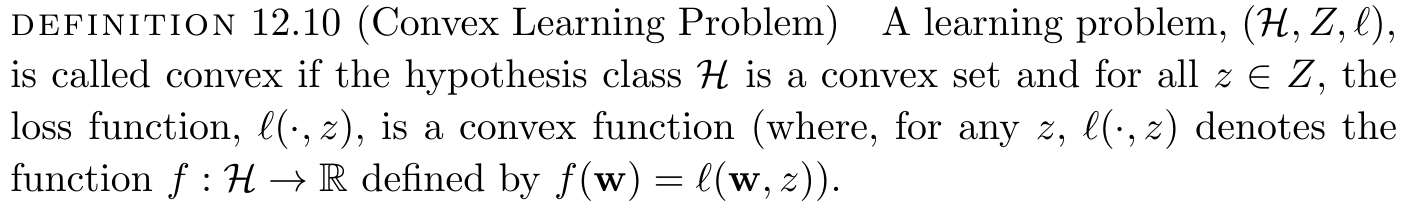
\includegraphics[scale=0.3]{def_12_10}
\end{figure}

\end{frame}

\begin{frame}
\frametitle{Convex Learning Problems: Intro}

Example 12.7: \\
Linear Regression with the Squared Loss
\begin{itemize}
    \item  to learn a linear function $h: \mathbb{R}^d \mapsto \mathbb{R}$ that best approximates
        the relationship between ``explanatory'' and outcome variables.
    \item Each linear function is parameterized by a vector $\mathbf{w} \in \mathbb{R}^d$,\\
        hence $\mathcal{H} = \mathbb{R}^d$
    \item set of examples:
    $\mathcal{Z} = \mathcal{X} \times \mathcal{Y} = \mathbb{R}^d \times \mathbb{R} = \mathbb{R}^{d+1}$
    \item loss function: $\ell(\mathbf{w}, (\mathbf{x}, y)) = (-y)^2$
    \item Clearly: $\mathcal{H}$ is a convex set and  $\ell$ is convex fn wrt $\mathbf{w}$
\end{itemize}

\begin{figure}
    \centering
    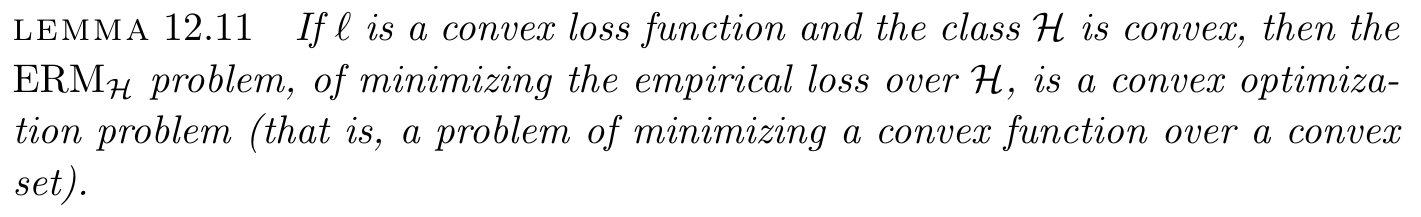
\includegraphics[scale=0.3]{lemma_12_11}
\end{figure}

\end{frame}

\begin{frame}
\frametitle{Convex Learning Problems: Learnability}
QUESTIONS:
\begin{itemize}
    \item is convexity a sufficient condition for the learnability of a problem?
    \item are all convex learning problems over $R^d$ learnable?
\end{itemize}
\vspace{5mm}

ANS:\\
\begin{itemize}
    \item \textbf{not all} convex learning problems over $\mathbb{R}^d$ are learnable.
    \item Convex problems are \textbf{learnable under} some restricting conditions:\\
        the properties of convexity, boundedness, and Lipschitzness or smoothness
        of the loss function are sufficient for learnability.
\end{itemize}

\end{frame}

\begin{frame}
\frametitle{Convex Learning Problems: Learnability}
TWO families of learning problems are learnable.

\noindent\makebox[\linewidth]{\rule{\paperwidth}{0.4pt}}

\begin{figure}
    \centering
    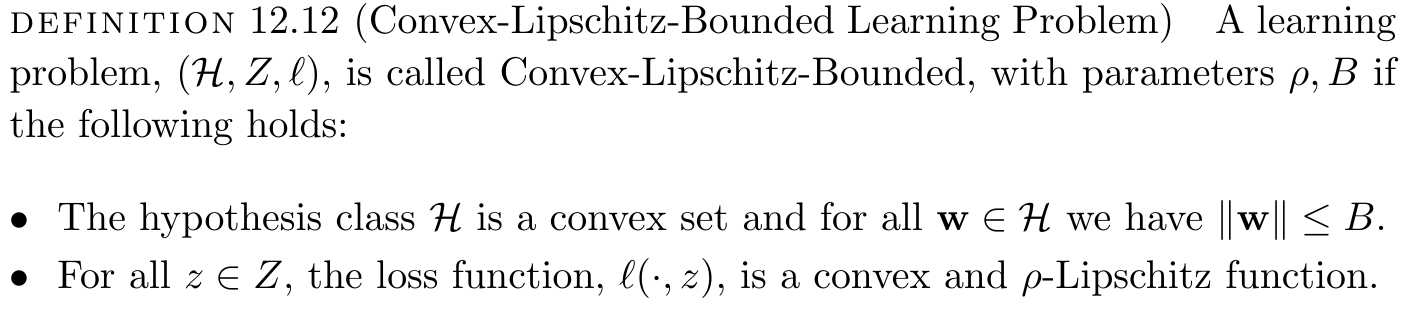
\includegraphics[scale=0.3]{def_12_12}
\end{figure}

\noindent\makebox[\linewidth]{\rule{\paperwidth}{0.4pt}}

\begin{figure}
    \centering
    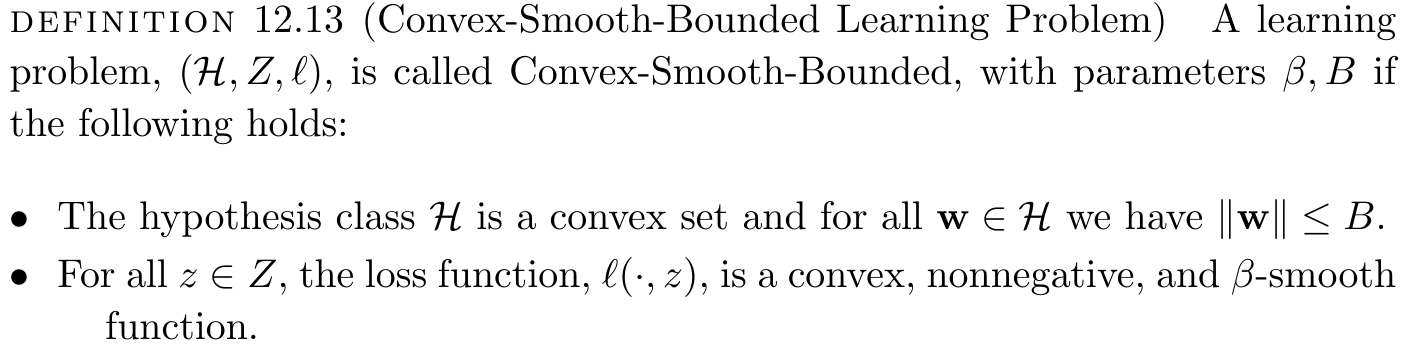
\includegraphics[scale=0.3]{def_12_13}
\end{figure}

\end{frame}


